\subsection{Flowcharts des fonctions clé}

\subsection*{getSubtree}

Comme déjà légèrement présenté dans la section \ref{sec:classes} \autoref{fig:ssimple-flowchart}, la fonction \texttt{getSubtree} est une fonction qui retourne un Subtree demandé. La fonction n'est pas statique car des paramètres spécifiques à la tailles des Subtrees comme \texttt{subtreeLevels}, le nombre de niveau dans un Subtree (cf. \autoref{fig:subtree-hierarchy}), et \texttt{maxLevels}, le nombre total de niveaux, doivent être connus au préalable.

Cette fonction de la classe \texttt{TdSubtreeStore}\footnote{org/apache/baremaps/tdtiles/TdSubtreeStore.java} est la seule fonction appelable par l'utilisateur. Les deux fonction ci-dessous, \texttt{createMaxRankSubtree} et \texttt{createSubtree}, sont des fonctions internes à la création d'un Subtree qui ne peuvent pas être appelées dans un autre context.

Pour être demandé, l'index du Subtree doit correspondre un index \textit{root} (cf. \autoref{fig:subtree-hierarchy}, \textit{Root tile of Subtree}) uniquement. Si le Subtree à l'index demandé existe dans la database existe, alors la fonction le retourne directement. Sinon, en fonction de si le Subtree demandé est un Subtree de rang maximal ou non, la fonction \texttt{createMaxRankSubtree} ou \texttt{createSubtree} sera appelée. Finalement, la fonction transforme le Subtree en un objet JSON binaire, met à jour la database et le retourne. La transformation en JSON binaire sera décrite dans la section \ref{sec:transmission}.

\begin{figure}[H]
    \centering
    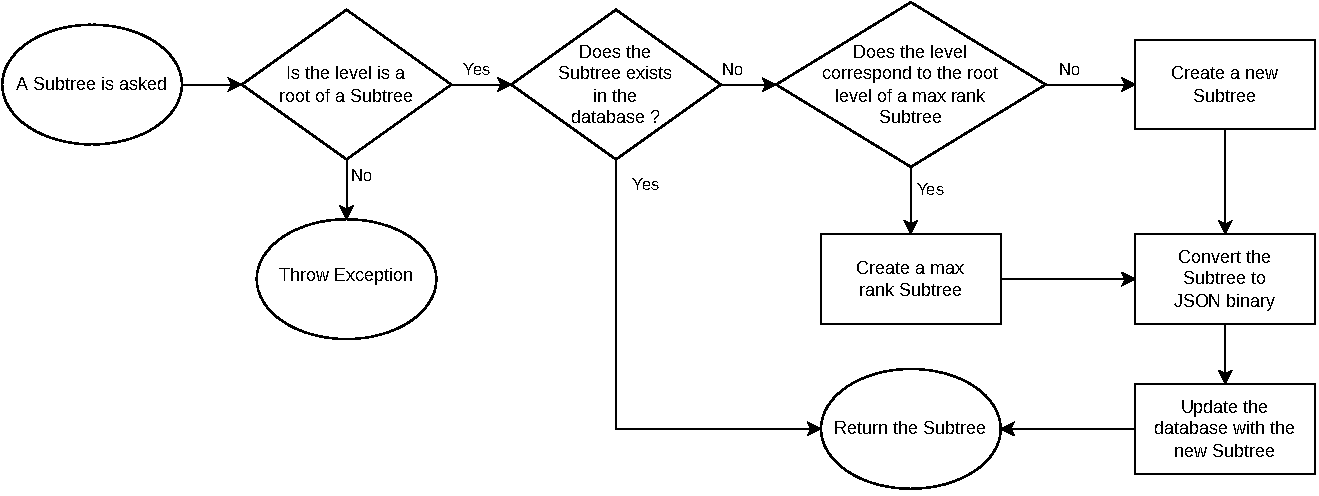
\includegraphics[width=1\textwidth]{assets/figures/getSubtree-flowchart.drawio.pdf}
    \caption{Flowchart de la fonction \texttt{getSubtree}}
    \label{fig:getsubtree-flowchart}
\end{figure}

\newpage
\subsection*{createMaxRankSubtree}

Cette fonction se charge uniquement de la création d'un Subtree de rang maximal. Un rang maximal est un Subtree qui se trouve à la fin de la hiérarchie de Subtrees, soit une feuille de l'arbre des Subtrees (cf. l'échelle de gauche sur la \autoref{fig:subtree-hierarchy}).

Pour commencer, si aucun bâtiments ne se trouve dans la zone de la tuile racine du Subtree, alors la fonction retourne un Subtree vide mais qui aura tout de même des objets Availability de bonne longueur et un nombre de levels correct. Sinon, la fonction va commencer par créer un BitSet qu'il remplira en parcourant toutes les tuiles de son niveau maximal (les plus petites tuiles qu'il contient). Si la tuile feuille contient des bâtiments, alors le BitSet sera mis à 1 à l'index de Motron local qui correspond à la tuile. Une fois que toutes les tuiles on été parcourues, la fonction va demander à la classe Availability de générer deux objets différents Availability à partir de ce BitSet, un pour la disponibilité des tuiles et un pour la disponibilité du contenu. En ce qui consiste la liste de disponibilité des enfants du Subtree, elle doit être vide. La fonction créé donc un Availability vide de la bonne longueur pour cette liste. Finalement, la fonction retourne un Subtree avec les trois Availability générés.

\begin{figure}[H]
    \centering
    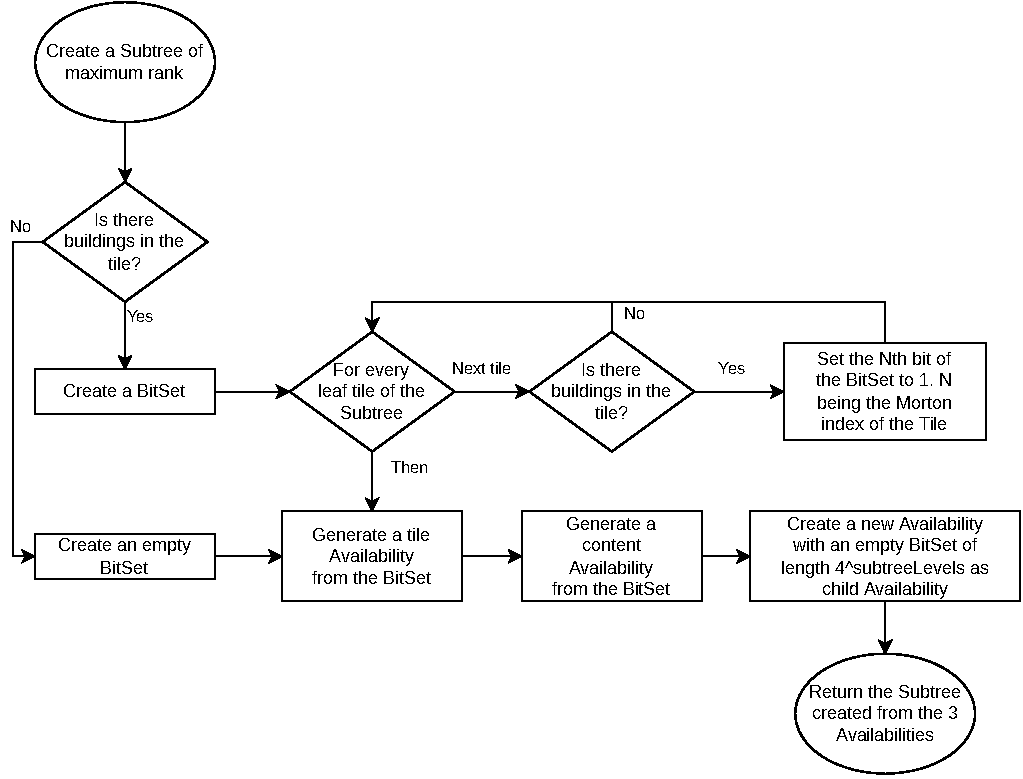
\includegraphics[width=1\textwidth]{assets/figures/maxRank-flowchart.drawio.pdf}
    \caption{Flowchart de la fonction \texttt{createMaxRankSubtree}}
    \label{fig:maxrank-flowchart}
\end{figure}

\newpage
\subsection*{createSubtree}

La fonction \texttt{createSubtree} est légèrement similaire à \texttt{createMaxRankSubtree} dans le sens qu'elle retourne aussi un Subtree sauf qu'elle ne s'occupe que des Subtree n'étant pas de rang maximal. Une autre similarité est que si aucun bâtiments ne se trouve dans la zone de la tuile racine du Subtree, alors la fonction retourne un Subtree vide.

Là où la fonction diffère est qu'elle se base sur le mécanisme de récursivité et de concaténation pour créer les Subtrees. Pour un Subtree demandé, la fonction va commencer par créer des Subtrees feuilles, du dernier niveau du Subtree demandé, puis les concaténer pour créer les Subtrees de niveau supérieur. On distingue donc deux cas de subtrees demandés :

    \noindent\hspace*{\fill}\parbox{0.9\textwidth}{\textbf{Subtree ayant plusieurs niveaux} : Ce sont les Subtrees qui ne sont pas des feuilles du Subtree demandé initialement. Pour le créer, la fonction va donc s'appeler elle-même pour créer les Subtrees de niveau inférieur, puis les concaténer pour créer le Subtree demandé.
    }

    \noindent\hspace*{\fill}\parbox{0.9\textwidth}{\textbf{Subtree ayant un seul niveau} : Ce sont les Subtrees qui sont des feuilles du Subtree demandé initialement. La fonction va tout d'abord créer une liste de 4 Subtrees. Ensuite, pour chacun de ces 4 Subtrees, il y a de nouveau deux cas :
    }

        \noindent\hspace*{\fill}\parbox{0.8\textwidth}{\textbf{On veut générer tous les Subtrees du Tileset} : En fonction de si ces 4 prochains Subtrees en dessous de cette feuille sont de rang maximal ou non, la fonction va appeler \texttt{createMaxRankSubtree} ou à nouveau \texttt{createSubtree} en demandant un Subtree complet pour les créer.
        }

        \noindent\hspace*{\fill}\parbox{0.8\textwidth}{\textbf{On ne veut générer que les Subtrees nécessaires} : La fonction commence simplement par regarder si il y a des bâtiments dans les tuiles de ce niveau. Si ce n'est pas le cas, elle créera 4 Subtrees vides. Sinon, elle va créer un Availability pour la disponibilité des tuiles de longueur 1 ayant une valeur de 1. Pour l'Availability de contenu, si les Subtrees inférieurs sont de rang maximal, alors elle créera aussi un Availability de longueur 1 ayant une valeur de 1, sinon de valeur 0. En ce qui concerne la liste de disponibilité des enfants du Subtree, elle peut être ignorée puisqu'elle disparaîtra lors de la concaténation.
        }

    Finalement, la fonction va concaténer les 4 Subtrees créés, update la database avec le résultat de la concaténation et retourner le Subtree demandé simplifié.

\begin{figure}[H]
    \centering
    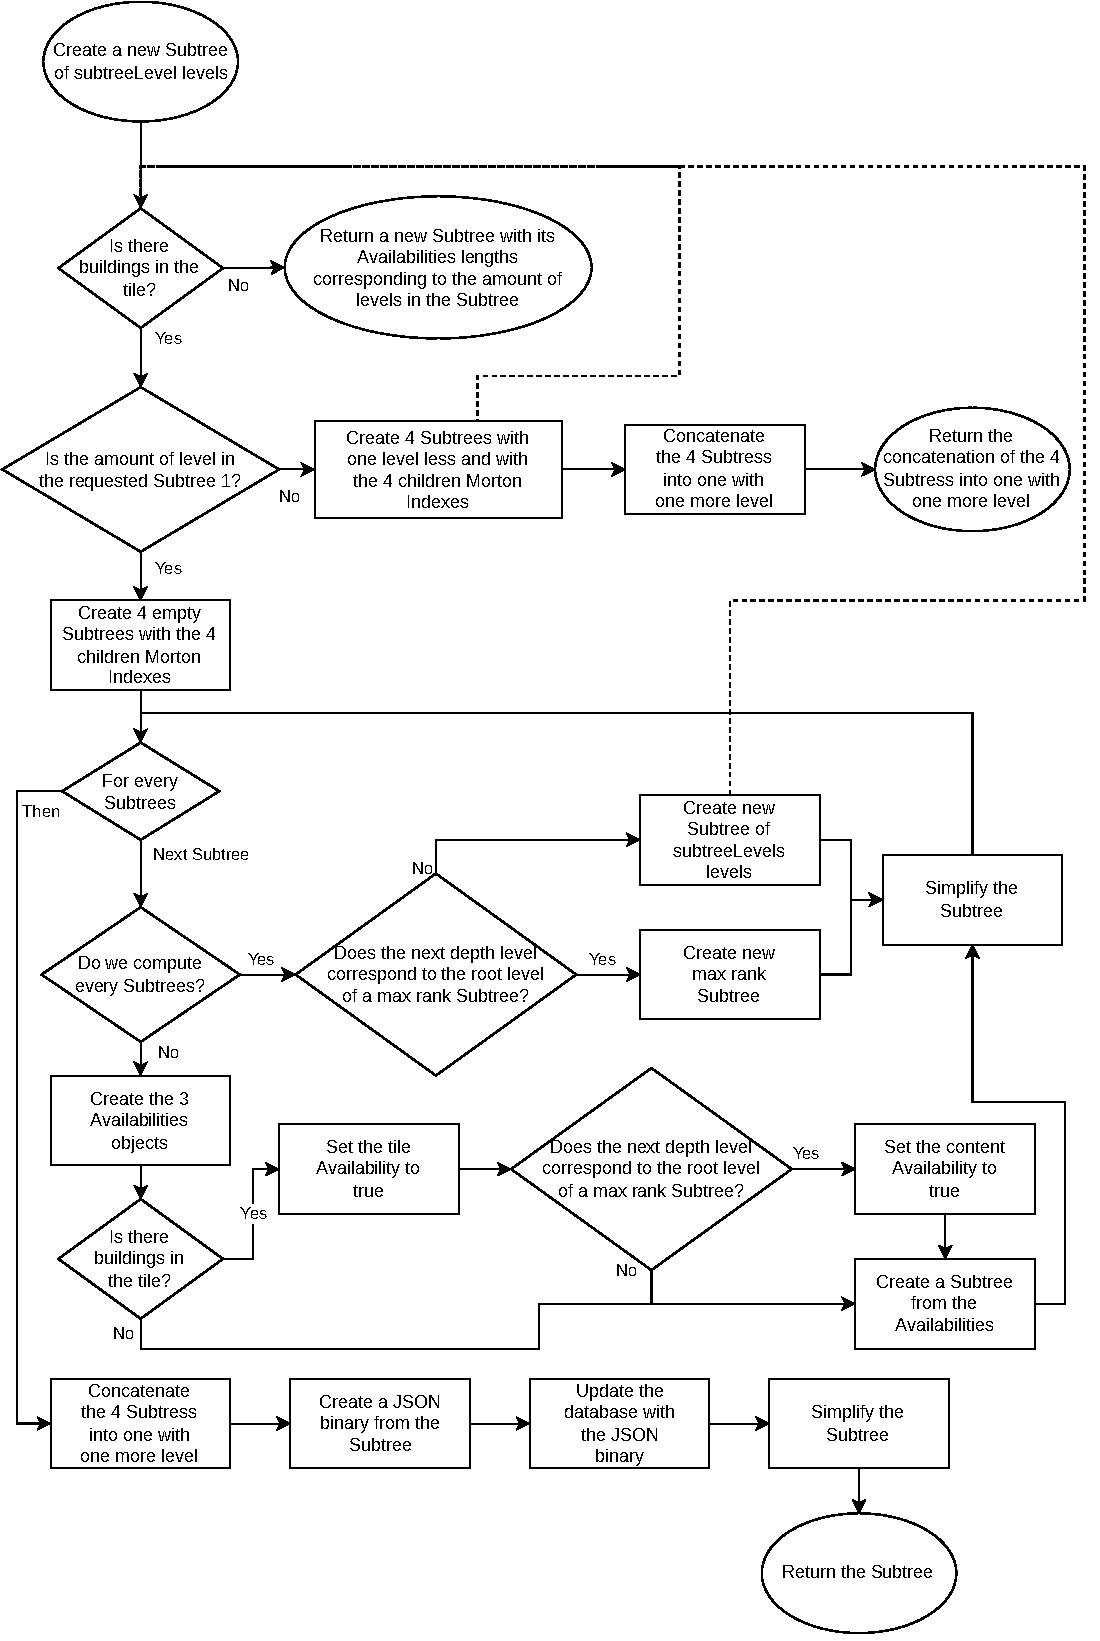
\includegraphics[width=1\textwidth]{assets/figures/createSubtree-flowchart.drawio.pdf}
    \caption{Flowchart de la fonction \texttt{createSubtree}}
    \label{fig:createsubtree-flowchart}
\end{figure}

\newpage
\subsection{Génération de Availability}
\label{sec:availability-gen}

Dans la fonction \texttt{createMaxRankSubtree}, deux objets Availability sont générés à partir d'un BitSet. Il faut donc trouver les autres BitSets de niveau supérieur à partir du BitSet donné.

\begin{figure}[H]
    \centering
    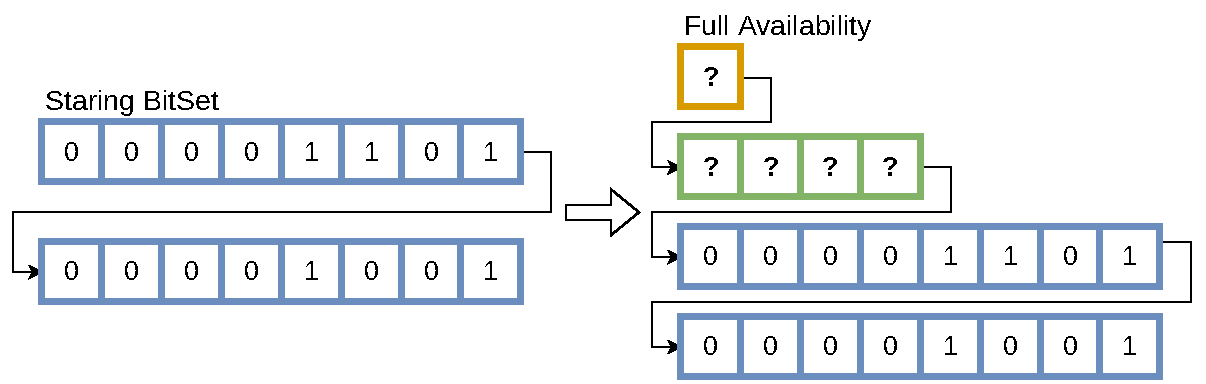
\includegraphics[width=1\textwidth]{assets/figures/availability-gen1.drawio.pdf}
    \caption{Génération de Availability : État initial}
    \label{fig:availability-gen1}
\end{figure}

Cela peut être fait en effectuant une opération \texttt{OR} sur chaque groupe de 4 bits du BitSet. Les bits du BitSet de niveau supérieur sont les résultats de ces opérations. On répète ensuite cette opération pour chaque niveau supérieur jusqu'à atteindre le niveau maximal.

\begin{figure}[H]
    \centering
    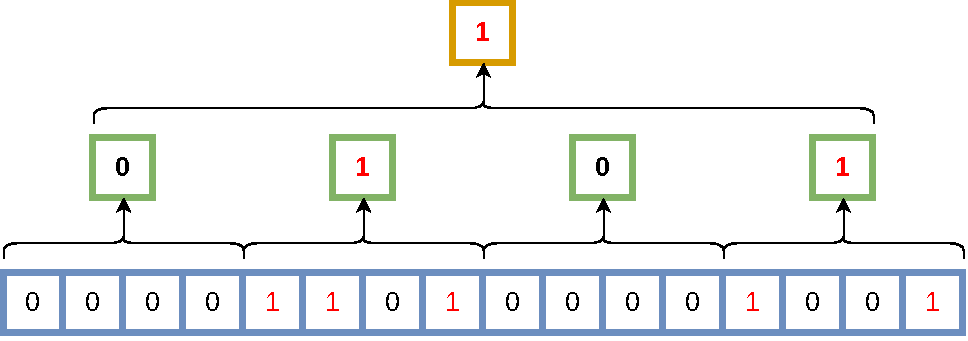
\includegraphics[width=1\textwidth]{assets/figures/availability-gen2.drawio.pdf}
    \caption{Génération de Availability : Procédure}
    \label{fig:availability-gen2}
\end{figure}

\newpage
\subsection{Concaténations}

Les concaténations de Subtrees sont effectuées fréquemment dans la fonction \texttt{createSubtree}. Elles consistent à diviser 4 objets Availability en BitSets par niveau. Ces BitSets sont ensuite concaténés pour former un seul BitSet par niveau. On se retrouve alors avec un un seul objet Availability ayant un niveau de plus que les objets initiaux, mais il lui manque encore le BitSet de taille 1 au niveau 0. Pour le créer, on peut simplement effectuer une opération \texttt{OR} sur les 4 BitSets de niveau 1.

\begin{figure}[H]
    \centering
    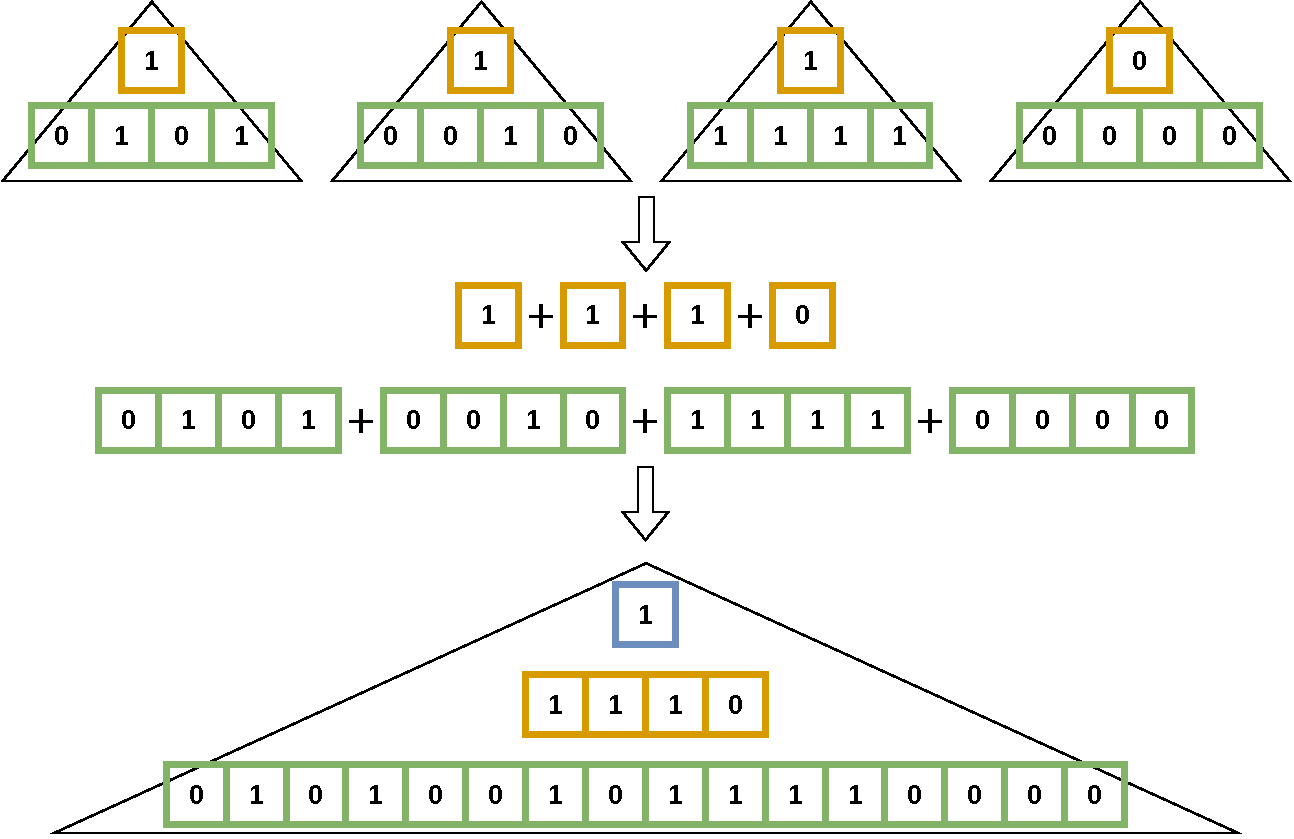
\includegraphics[width=1\textwidth]{assets/figures/availability-concat.drawio.pdf}
    \caption{Concaténation de 4 Availability}
    \label{fig:availability-concat}
\end{figure}

